% -- Proyecto Ars_Mathematica
% https://www.instagram.com/ars_mathematica/
%
% Autor:		Rodrigo Sánchez-Martínez
% Fecha:		30 de mayo del 2024
% Contacto:		rodrigo.smtz@icloud.com
%
% Descripción de la figura:
% 	Diagrama de Feynman que representa la interacción entre dos Fermiones via su momento dipolar.
%	Reproducción propia, tomada de la figura 1 de la referencia:
%		"Dipoles in quantum field theory" Am. J. Phys. 87, 146 (2019)
%
% Licencia:
%	Este código puede ser distribuido libremente.
%	El objetivo de este proyecto es compartir con ustedes un poco de las herramientas que utilizo en TikZ y que he aprendido con la experiencia.
%	Por favor, no duden en contactarme si tienen alguna duda o si hay algun error tanto en la parte del código de LaTeX, como en la descripción matemática y física de los conceptos.
%
%	Rodrigo.

\documentclass[border = 1mm]{standalone}

% -- Paqueterías importantes

% entrada
\usepackage[utf8]{inputenc}
% matemáticas
\usepackage{amsmath}

% TikZ
\usepackage{tikz}
\usetikzlibrary{
	math, calc,
	patterns.meta, arrows.meta,
	decorations.markings, decorations.pathmorphing
}

% Tamaño del dibjo completo
\def\L{6} % cm

% -- Cuerpo del documento
\begin{document}

%
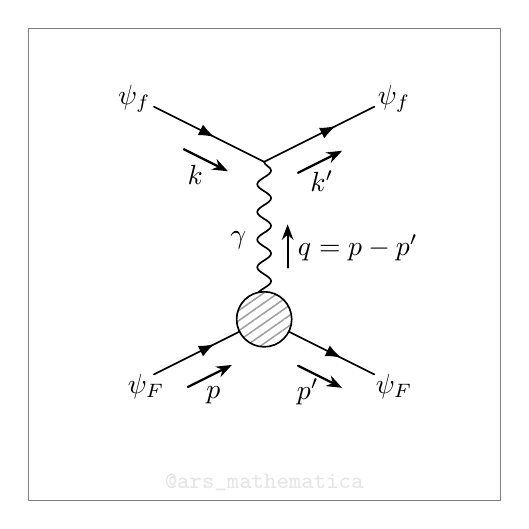
\begin{tikzpicture}[
	% Propiedades generales del dibujo
	line join = round, line cap = round,
	% Definición de nuevos estilos
	% 	a. fotón
	photon/.style = {
		decoration = snake,
		decorate
	},
	% 	b. fermión:
	%		el argumento #1 indica la posición relativa
	%		de la punta de flecha
	fermion/.style = {
		decoration = {
    		markings,
    		mark = at position #1 with {\arrow{Latex}}
    	},
    	postaction = {decorate}
	},
	%	c. vértices de interacción
	interaction/.style = {
		pattern = {Lines[angle = 35, line width = 0.55pt]},
		pattern color = gray!75,
		preaction = {fill = white}
	},
	%	d. vector
	vector/.style = {
		thick,
		arrows = -{Stealth[scale = 0.85]},
	},
]

	% márgenes del dibujo
	\draw[help lines] (0,0) rectangle (\L,\L);

	% desplazamiento del origen de coordenadas al centro de la imagen
	\begin{scope}[
		shift = {(0.5*\L, 0.55*\L)}
	]

		% definición de las variables
		\tikzmath{
			\sep{y} = 2.0; % sep. vertical de los vértices
			\sep{x} = 2.8; % sep. horizonal de los vértices
		}

		% def. de las coordenadas importantes
		\coordinate (a1) at (-0.5*\sep{x},+0.85*\sep{y}); % psi_f
		\coordinate (a2) at (+0.5*\sep{x},+0.85*\sep{y}); % psi_f
		
		\coordinate (v1) at (0,+0.5*\sep{y}); % vértice sup.
		\coordinate (v2) at (0,-0.5*\sep{y}); % vértice inf.
	
		\coordinate (b1) at (-0.5*\sep{x},-0.85*\sep{y}); % psi_F
		\coordinate (b2) at (+0.5*\sep{x},-0.85*\sep{y}); % psi_F
		
		% fermiones
		\draw[semithick, fermion = 0.55]
			(b1)
				node[shift = {(-1mm,-1.5mm)}] {$\psi_F$}
			-- (v2);
			
		\draw[semithick, fermion = 0.70]
			(v2) -- (b2)
				node[shift = {(2.5mm,-1.5mm)}] {$\psi_F$};
		
		\draw[semithick, fermion = 0.55]
			(a1) 
				node[shift = {(-2.5mm,+1mm)}] {$\psi_f$}
			-- (v1);
			
		\draw[semithick, fermion = 0.65]
			(v1) -- (a2)
				node[shift = {(+2.5mm,+1mm)}] {$\psi_f$};

		% coordenada temporal que me permite despazar los vectores
		% de manera paralela a las líneas de los fermiones
		\coordinate (tmp) at (0.15,-0.3);
		\draw[vector]
			($(b1)!0.2!(v2) + (tmp)$)
				-- node[pos = 0.4, shift = {(0.1,-0.22)}] {$p$}
			($(b1)!0.6!(v2) + (tmp)$);
			
		\coordinate (tmp) at (0.15,-0.45);
		\draw[vector]
			($(v2)!0.2!(b2) + (tmp)$)
				-- node[pos = 0.4, shift = {(-0.1,-0.22)}] {$p'$}
			($(v2)!0.6!(b2) + (tmp)$);
			
		\coordinate (tmp) at (0.1,-0.40);
		\draw[vector]
			($(a1)!0.2!(v1) + (tmp)$)
				-- node[pos = 0.4, shift = {(-0.08,-0.22)}] {$k$}
			($(a1)!0.6!(v1) + (tmp)$);
			
		\coordinate (tmp) at (0.15,-0.28);
		\draw[vector]
			($(v1)!0.2!(a2) + (tmp)$)
				--node[pos = 0.4, shift = {(0.08,-0.22)}] {$k'$}
			($(v1)!0.6!(a2) + (tmp)$);

		% fotón
		\draw[semithick, photon]
			(v1) --
				node[left = 1mm] {$\gamma$}
				node[right = 1mm, pos = 0.54] {
					\tikz[line cap = round]{
						\draw[vector]
							(0,0) --
								node[right, pos = 0.45] {$q = p - p'$} 
							(0,0.55);
				}}
			(v2);
		
		% interacción
		\draw[semithick, interaction] (v2) circle (0.35);
		
	\end{scope}

	% marca de agua
	\node[above, scale = 0.95, opacity = 0.1]
		at (0.5*\L,0)
		{\small\verb|@ars_mathematica|};

\end{tikzpicture}	
\end{document}